\centerline{\bf \huge 9 класс}
\centerline{\bf \huge Решения}

\problem{1}
Эвена сложила десять подряд идущих натуральных чисел, затем разделила полученную сумму на сумму следующих десяти натуральных чисел. Могло ли у неё получится число $0,8 ?$
%Москва 2017

\textbf{Ответ: не могло.}

\textbf{Решение.} 
Предположим, что при делении получилось 0,8 . Обозначим наименьшее число первой суммы через $n$. Тогда эта сумма равна: $n+(n+1)+\ldots+(n+9)=10 n+45$. Каждое слагаемое второй суммы на 10 больше соответствующего слагаемого первой суммы, поэтому вторая сумма на 100 больше, чем первая.

Таким образом, $\frac{10 n+45}{10 n+145}=\frac{4}{5}$. Преобразуя это равенство, получим, что $n=35,5$. Это противоречит тому, что $n$ - натуральное число.


\problem{2}
Известно, что сумма квадратов корней квадратного уравнения $x^2+b x+ c=0$ равна 2023. Найдите сумму квадратов корней $x^2+b x+c=\frac{1}{2}$.
%Ростов 2023

\textbf{Ответ: 2024}

\textbf{Решение.}
Пусть $x_1, x_2$ - корни квадратного уравнения $x^2+b x+c=0$, тогда $x_1+x_2=-b, x_1 x_2=c$. Так как $x_1^2+x_2^2=\left(x_1+x_2\right)^2-2 x_1 x_2= b^2-2 c$, то $b^2-2 c=2023$. Пусть $x_3, x_4$ - корни квадратного уравнения $x^2+b x+c-\frac{1}{2}=0$, тогда $x_3^2+x_4^2=\left(x_3+x_4\right)^2-2 x_3 x_4=b^2-2\left(c-\frac{1}{2}\right)= b^2-2 c+1=2023+1=2024$.

\problem{3}
В таблицу $4 \times 4$ записали натуральные числа. Могло ли оказаться так, что сумма чисел в каждой следующей строке на 2 больше, чем в предыдущей, а сумма чисел в каждом следующем столбце на 3 больше, чем в предыдущем?
%Ставрополь 2017    

\textbf{Ответ: не могло}

\textbf{Решение}
Предположим, что такое возможно. Пусть сумма чисел в первой строке равна $a$, а сумма чисел в первом столбце равна $b$. Тогда сумма всех чисел в таблице равна $a+(a+2)+(a+4)+(a+6)=4 a+12$, то есть кратна 4 . С другой стороны, она же равна $b+(b+3)+(b+6)+(b+9)=4 b+18$, то есть не кратна 4. Противоречие.

\problem{4}
В одну из вершин шестиугольника Скрудж МакДак положил золотую монетку, а в остальных вершинах ничего нет. Каждый день он убирает с одной из вершин шестиугольника произвольное количество монеток и тут же кладёт на соседнюю вершину в шесть раз больше монеток. Если в какойто день Скрудж МакДак сможет добиться того, что во всех вершинах шестиугольника одинаковое число монеток, то ему будет присвоено звание «Великий Селезень». Сможет ли Скрудж МакДак получить это звание?
%Красноярск 2017

\textbf{Ответ: Не сможет.}

\textbf{Решение.}
Занумеруем вершины шестиугольника, начиная с той, где лежит монетка, последовательными натуральными числами от 1 до 6 (двигаясь, например, против часовой стрелки). Обозначим через $n_1, n_2, \ldots, n_6$ - количества монеток, лежащих в вершинах $1,2, \ldots, 6$ соответственно. Пусть $N_1=n_1+n_3+n_5, N_2=n_2+n_4+n_6$. Рассмотрим разность $N_1-N_2$ и докажем, что при указанных действиях Скруджа МакДака остаток от ее деления на 7 не изменяется. Действительно, если из какой-то вершины шестиугольника Скрудж МакДак забирает $x$ монеток, а в соседнюю вершину добавляет $6 x$ монеток, то значение $N_1-N_2$ изменяется на $7 x$. Заметим, что в начальный момент $N_1- N_2=1$. Поэтому цель Скруджа МакДака - уравнять количество монеток во всех вершинах, а значит сделать так, чтобы $N_1-N_2$ было равно нулю, - недостижима.

\problem{5}
В прямоугольном треугольнике $A B C\left(\angle C=90^{\circ}\right)$ внутри отрезка $B C$ расположена точка $D, C P$ и $C Q$ - высоты треугольников $A B C$ и $A D C$ соответственно. Докажите, что треугольники $A P Q$ и $A D B$ подобны.
%Краснодар 2017

\textbf{Решение.}
Так как $\angle A P C=\angle A Q C=90^{\circ}$, то окружность построенная на стороне $A C$ как на диаметре пройдет через точки $Q$ и $P$. Вписанные углы в эту окружность $A C P$ и $A Q P$ равны, так как опираются на одну и ту же дугу. Треугольники $A P C$ и $A C B$ подобны по двум углам, поэтому $\angle A C P=\angle A B C$. Откуда следует, что $\angle A Q P=\angle A B D$. Тогда треугольники $A P Q$ и $A D B$ подобны по двум углам.

\begin{center}
    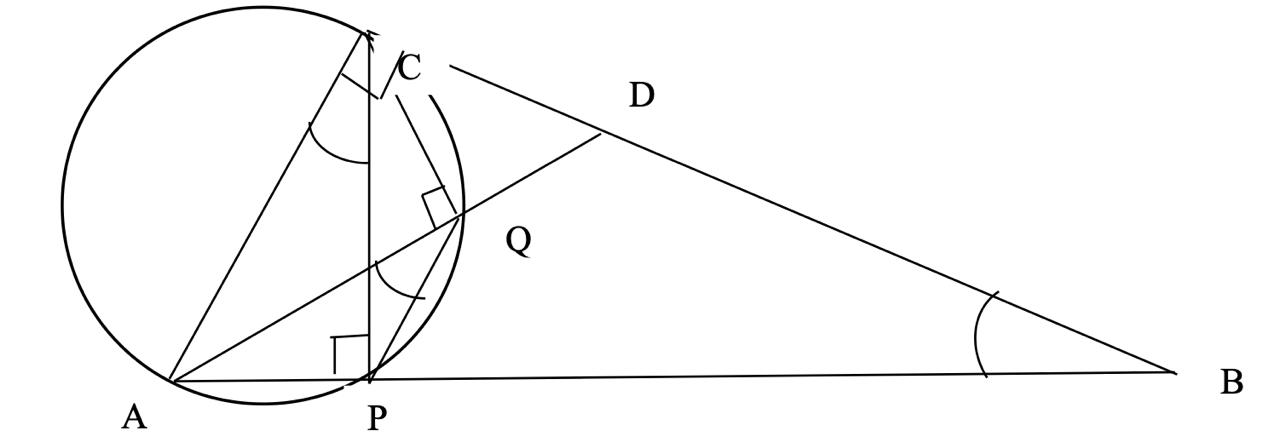
\includegraphics[width=0.7\textwidth]{ЭлМШ 2025-2026/III блок/10/Тренировки/I/Решения/9.5.jpg}
\end{center}
